\begin{figure}[t]
  \centering
  \begin{subfigure}[t]{0.32\linewidth}
    \centering
    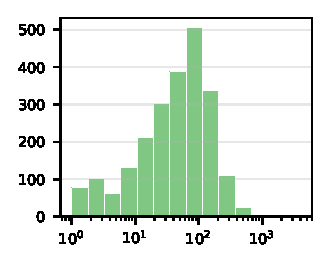
\includegraphics[width=\linewidth]{images/pr_lean_added_hist_compact.pdf}
    \subcaption{\small Added lines}
    \label{fig:hist-add}
  \end{subfigure}\hfill
  \begin{subfigure}[t]{0.32\linewidth}
    \centering
    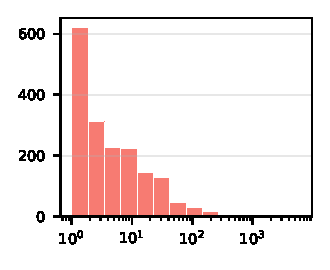
\includegraphics[width=\linewidth]{images/pr_lean_deleted_hist_compact.pdf}
    \subcaption{\small Removed lines}
    \label{fig:hist-del}
  \end{subfigure}\hfill
  \begin{subfigure}[t]{0.32\linewidth}
    \centering
    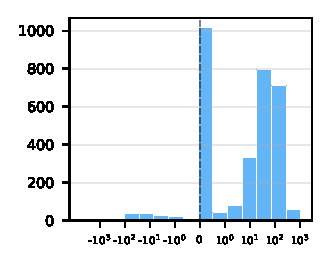
\includegraphics[width=\linewidth]{images/pr_lean_net_hist_compact.pdf}
    \subcaption{\small Net change}
    \label{fig:hist-net}
  \end{subfigure}
  \caption{\textbf{Histograms of agent PR line counts.}
  The histograms show the number of agents that return within a given range of added, removed or net added lines. 
  The multi-agent setup ensures that pull requests are granular and atomic, comprising around 100 lines.
  Refactorings that reduce the overall code size are rare, but PRs frequently replace code while extending the code base overall.
  }
  \label{fig:hists}
\end{figure}
